% -*- TeX-engine: luatex -*-
\documentclass[dvipsnames,presentation,aspectratio=169,14pt]{beamer}
\usepackage{hastingstheme}
\titlegraphic{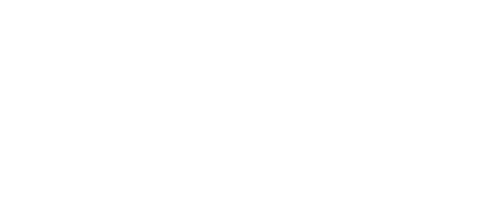
\includegraphics[scale=.35]{static_figures/du_bn.pdf}}
\author{\large Massimiliano Fasi}
\date{}


% \usepackage{template}
% \renewcommand{\authorname}{Lawrence Mitchell\inst{*}}
\renewcommand{\authoremail}{\inst{*}\texttt{lawrence.mitchell@durham.ac.uk}}

% \renewcommand{\sessionnumber}{5}
% \renewcommand{\sessiontitle}{Cache blocking/tiling}
% \usepackage{tikz}

\usetikzlibrary{matrix,fit,positioning,calc}
\usepackage{pgfplotstable}
\usepackage{booktabs}
\usetikzlibrary{pgfplots.groupplots}
\date{}

\begin{document}

\title{\firasemibold\color{White}%
  {\fontsize{20}{0}\selectfont SESSION 6\\
    \fontsize{34}{34}\selectfont Cache blocking\\\& tiling\par}}
\titleslide

\begin{frame}[fragile]
\frametitle{Computing the matrix transpose}
Given $N$-by-$N$ matrices $A$ and $B$, we can compute
\begin{equation*}
  B_{ij} \gets A_{ji}
\end{equation*}
with
\begin{minted}{c}
  double *A, *B;
  ...
  for (int i = 0; i < N; i++)
    for (int j = 0; j < N; j++)
      B[i*N + j] = A[j*N + i];
\end{minted}
\pause
\vskip 11pt


\structure{What is the performance of this code?}
\end{frame}

\begin{frame}
  \frametitle{Matrix transpose: simple performance model}
  \begin{columns}
    \begin{column}{.4\textwidth}
      \begin{itemize}[wide=0pt,itemsep=14pt]
      \item $N^\mathsf{2}$ stores
      \item $N^\mathsf{2}$ loads
      \item no computation
      \end{itemize}
      \vskip 11pt

      \structure{What do you expect?}
    \end{column}
    \pause
    \begin{column}{.55\textwidth}
      \begin{center}
        \begin{tabular}{cc}
          \toprule
          Matrix size & bandwidth [GB/s]\\
          \midrule
          $\mathsf{128\times 128}$ & 22\phantom{.6}\\
          $\mathsf{256 \times 256}$ & 13\phantom{.0}\\
          $\mathsf{512 \times 512}$ & 13\phantom{.0}\\
          $\mathsf{1024 \times 1024}$ & \phantom{0}5\phantom{.0}\\
          $\mathsf{2048 \times 2048}$ & \phantom{0}1.6\\
          $\mathsf{4096 \times 4096}$ & \phantom{0}0.9\\
          \bottomrule
        \end{tabular}
      \end{center}
    \end{column}
  \end{columns}
\end{frame}

\begin{frame}[fragile]
  \frametitle{What went wrong?}

  \begin{center}
\begin{minted}{c}
            for (int i = 0; i < N; i++)
                for (int j = 0; j < N; j++)
                    B[i*N + j] = A[j*N + i];
\end{minted}
    \vskip 5pt

  \end{center}
  \begin{itemize}[itemsep=8pt]
  \item Contiguous access to \texttt{B}, stride-$N$ access to \texttt{A}

  \item If both matrices fit in cache, a reasonable model could be
    \begin{equation*}
    T_{\text{cache}} = N^{\mathsf{2}}(t_\text{read} + t_\text{write})
  \end{equation*}

  \item Reads of \texttt{A} load a full cache line, but use only 8 bytes:
    \begin{equation*}
       T_\text{mem} = N^{\mathsf 2}(\mathsf 8 t_\text{read} + t_\text{write})
    \end{equation*}
  \end{itemize}
\end{frame}

\begin{frame}
  \frametitle{A picture}
  \begin{columns}
    \begin{column}{0.45\textwidth}
      \begin{center}
        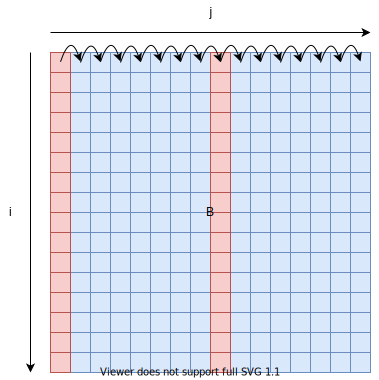
\includegraphics[width=\textwidth]{figures/strideoneaccess.png}
      \end{center}
    \end{column}
    \begin{column}{0.45\textwidth}
      \begin{center}
        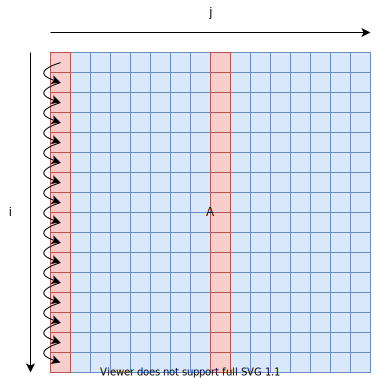
\includegraphics[width=\textwidth]{figures/stridenaccess.png}
      \end{center}
    \end{column}
  \end{columns}
\end{frame}

\begin{frame}
  \frametitle{Cache locality}
  \begin{itemize}
  \item Matrices are stored by rows
  \item Cache line size is $L$
  \item \texttt{A} has strided access
  \item We need $LN/\mathsf{8}$ cache to get reuse
  \item We can \emph{reorder} the iterations to preserve spatial locality
  \end{itemize}
  \begin{answer}{Idea}
    \begin{itemize}
    \item Break loop iteration space into blocks
      \begin{enumerate}[itemsep=6pt]
      \item \emph{strip mining}
      \item \emph{loop reordering}
      \end{enumerate}
    \end{itemize}
  \end{answer}
\end{frame}

\begin{frame}[fragile]
  \frametitle{Strip mining}
  \begin{challenge}{\small Before}
\begin{minted}{c}
  for ( int i = 0; i < N; i++ )
    A[i] = f(i);
\end{minted}
  \end{challenge}
  \vskip 6pt
  \begin{answer}{\small After}
\begin{minted}{c}
  for ( int ii = 0; ii < N; ii += stride)
    for ( int i = ii; i < min(N, ii + stride); i++)
      A[i] = f(i);
\end{minted}
  \end{answer}
  \vskip 6pt

  Mostly useful for nested loops
\end{frame}

\begin{frame}[fragile]
  \frametitle{Strip mining nested loops}
    \begin{challenge}{\small Before}
\begin{minted}{c}
  for (int i = 0; i < N; i++)
    for (int j = 0; j < N; j++)
      B[i*N + j] = A[j*N + i];
\end{minted}
    \end{challenge}

    \begin{answer}{\small After}
\begin{minted}{c}
  for (int ii = 0; ii < N; ii += stridei)
    for (int i = ii; i < min(N, ii+stridei); i++)
      for (int jj = 0; jj < N; jj += stridej)
        for (int j = jj; j < min(N, jj+stridej); j++)
          B[i*N + j] = A[j*N + i];
\end{minted}
    \end{answer}
% Haven't yet made any change to the performance
\end{frame}

\begin{frame}[fragile]
  \frametitle{Reordering loops}
  \begin{exampleblock}{\small After permuting \texttt{i} and \texttt{jj} loops}
\begin{minted}{c}
  for (int ii = 0; ii < N; ii += stridei)
    for (int jj = 0; jj < N; jj += stridej)
      for (int i = ii; i < min(N, ii+stridei); i++)
        for (int j = jj; j < min(N, jj+stridej); j++)
          b[i*N + j] = a[j*N + i];
\end{minted}
  \end{exampleblock}
  \begin{itemize}
  \item Two free parameters \texttt{stridei} and \texttt{stridej}
  \item Need to choose according cache hierarchy
  \item Ideally block for L1, L2, L3
  \item The extra logic adds some overhead
  \end{itemize}
\end{frame}

\begin{frame}
  \frametitle{Iteration over $B$}
  \begin{center}
    \begin{minipage}[t][\parskip][t]{0.4\textwidth}
      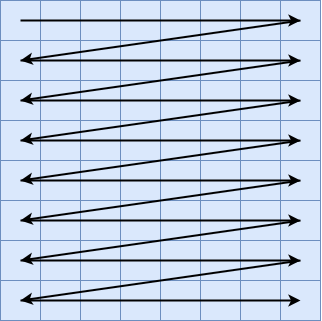
\includegraphics[width=\textwidth]{figures/originalrowmajororder.png}
      \centering

      Before
    \end{minipage}
    \qquad
    \begin{minipage}[t][\parskip][t]{0.4\textwidth}
      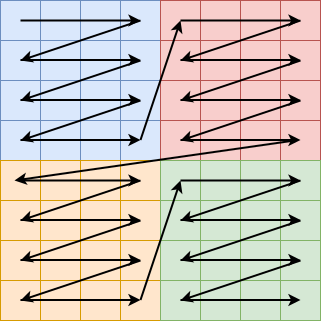
\includegraphics[width=\textwidth]{figures/tiledrowmajororder.png}
      \centering

      After
    \end{minipage}
  \end{center}
\end{frame}

\begin{frame}
  \frametitle{Iteration over $A$}
  \begin{center}
    \begin{minipage}[t][\parskip][t]{0.4\textwidth}
      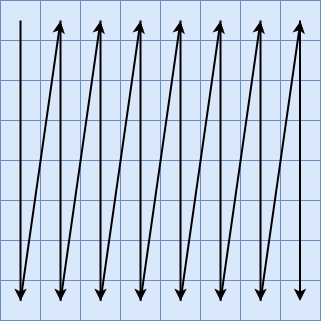
\includegraphics[width=\textwidth]{figures/originalcolmajororder.png}
      \centering

      Before
    \end{minipage}
    \qquad
    \begin{minipage}[t][\parskip][t]{0.4\textwidth}
      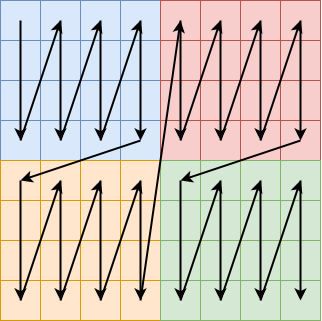
\includegraphics[width=\textwidth]{figures/tiledcolmajororder.png}
      \centering

      After
    \end{minipage}
  \end{center}
\end{frame}

\begin{frame}
  \frametitle{Comparison }
  \begin{center}
    \begin{minipage}[t][\parskip][t]{0.4\textwidth}
      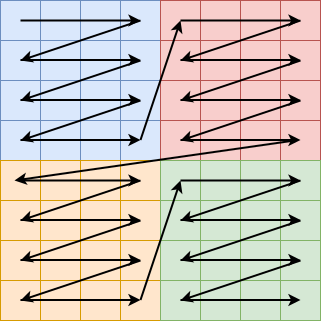
\includegraphics[width=\textwidth]{figures/tiledrowmajororder.png}
      \centering

      Tiled $B$
    \end{minipage}
    \qquad
    \begin{minipage}[t][\parskip][t]{0.4\textwidth}
      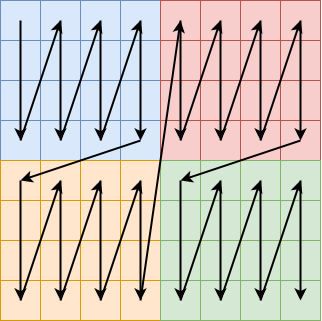
\includegraphics[width=\textwidth]{figures/tiledcolmajororder.png}
      \centering

      Tiled $A$
    \end{minipage}
  \end{center}
\end{frame}

\begin{frame}
  \frametitle{Exercise 7: Tiled matrix transpose}
  \begin{enumerate}[itemsep=8pt]
  \item Split into small groups
  \item Download the two versions of the code
  \item Measure bandwidth as matrix size changes
  \item Try different tile sizes
  \item Ask questions!
  \end{enumerate}
\end{frame}

\begin{frame}[fragile]
  \frametitle{Matrix--matrix multiplication}
  Given $n$-by-$n$ matrices $A$ and $B$, we can compute $C = AB$
  \begin{equation*}
    C_{ij} \gets C_{ij } + \sum_k A_{ik} B_{kj}
  \end{equation*}
  with
\begin{minted}[fontsize=\normalsize]{c}
          for (int i = 0; i < n; i++)
            for (int j = 0; j < n; j++)
              for (int k = 0; k < n; k++)
                C[i*n + j] += A[i*n + k] * B[k*n + j];
\end{minted}

  % Same story here (or at least it was in the 90s!).
\end{frame}


\begin{frame}
  \frametitle{(Another) simple model for computation}
  \begin{itemize}
  \item Simple model of memory, two levels: ``fast'' and ``slow''
  \item Initially all data in slow memory
    \begin{itemize}
    \item[$m$] number of data elements moved between fast and slow memory
    \item[$t_m$] time per slow memory operation
    \item[$f$] number of flops
    \item[$t_f \ll t_m$] time per flop
    \item[$q =: f/m$] average flops per slow memory access
    \end{itemize}
  \item Minimum time to solution (all data in fast memory)
    \begin{equation*}
      t_f f
    \end{equation*}
  \item Typical time
    \begin{equation*}
      f t_f + m t_m = f t_f \left(1 + \frac{t_m}{t_f}\frac{1}{q}\right)
    \end{equation*}

  \item $t_m / t_f$ property of hardware, $q$ property of \emph{algorithm}
  \end{itemize}
\end{frame}

\begin{frame}[fragile]
  \frametitle{Na\"ive matrix-multiply}
  \begin{onlyenv}<1>
\begin{minted}[fontsize=\scriptsize]{c}
for (int i = 0; i < n; i++)
  for (int j = 0; j < n; j++)
    for (int k = 0; k < n; k++)
      C[i*n + j] = C[i*n + j] + A[i*n + k] * B[k*n + j];
\end{minted}
    \begin{itemize}
    \item Algorithm does $2n^3 = \mathcal{O}(n^3)$ flops and touches
      $3\cdot 8 n^2$ bytes of memory
    \item $q$ potentially $\mathcal{O}(n)$, arbitrarily large for large $n$.
    \end{itemize}
  \end{onlyenv}
  \begin{onlyenv}<2>
\begin{minted}[fontsize=\scriptsize, mathescape=true]{c}
for (int i = 0; i < n; i++)
  // Read row $i$ of $A$ into fast memory
  for (int j = 0; j < n; j++)
    // Read $C_{ij}$ into fast memory
    // Read column $j$ of $B$ into fast memory
    for (int k = 0; k < n; k++)
      C[i*n + j] = C[i*n + j] + A[i*n + k] * B[k*n + j];
    // Write $C_{ij}$ back to slow memory
\end{minted}
  \end{onlyenv}
  \begin{onlyenv}<3>
    \begin{block}{Number of slow memory references}
      \vspace{-\baselineskip}
      \begin{align*}
        m &= n^3 \quad \text{each column of $B$ is read $n$ times}\\
          &+ n^2 \quad \text{each row of $A$ is read $n$ once}\\
          &+ 2n^2 \quad \text{each entry of $C$ is read once and
            written once}\\
          &= (n^3 + 3n^2)
      \end{align*}
      Hence
      \begin{equation*}
        \lim_{n\to \infty} q = \frac{f}{m} = \frac{2n^3}{(n^3 + 3n^2)} = 2
      \end{equation*}
    \end{block}
  \end{onlyenv}
  \begin{center}
    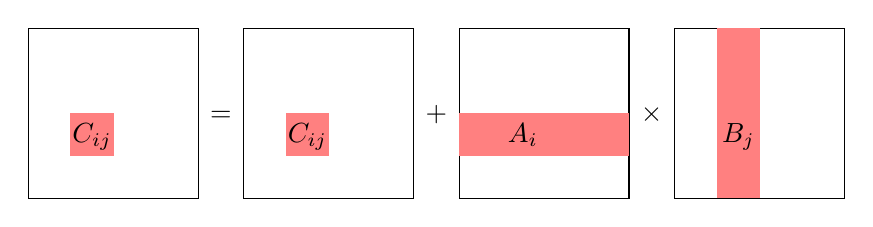
\begin{tikzpicture}[nodes in empty cells,
      inner sep=0cm,
      nodes={minimum width=0.55cm, minimum height=0.55cm, text
        height=0.35cm, text depth=0.15cm},
      row sep=-\pgflinewidth, column sep=-\pgflinewidth]
      \matrix(Cout)[draw, matrix of nodes]
      {
        & & & \\
        & & & \\
        &|[fill=red!50]| $C_{ij}$ & & \\
        & & & \\
      };
      \node[right=0cm of Cout] (eq) {$=$};
      \matrix(Cin)[right=0cm of eq, draw, matrix of nodes]
      {
        & & & \\
        & & & \\
        &|[fill=red!50]| $C_{ij}$ & & \\
        & & & \\
      };
      \node[right=0cm of Cin] (plus) {$+$};
      \matrix(Ain)[right=0cm of plus, draw, matrix of nodes,
      row 3/.style={nodes={fill=red!50}}]
      {
        & & & \\
        & & & \\
        & $A_{i}$ & & \\
        & & & \\
      };
      \node[right=0cm of Ain] (times) {$\times$};
      \matrix(Bin)[right=0cm of times, draw, matrix of nodes,
      column 2/.style={nodes={fill=red!50}}]
      {
        &  & & \\
        &  & & \\
        & $B_{j}$ & & \\
        & & & \\
      };
    \end{tikzpicture}
  \end{center}
\end{frame}

\begin{frame}
  \frametitle{From model to prediction}
  \begin{itemize}
  \item So for a triply-nested loop structure, the \emph{best} time to
    solution our model predicts is:
    \begin{equation*}
      T = t_f f \left(1 + \frac{t_m}{2 t_f}\right)
    \end{equation*}
  \item Recall that on modern hardware, memory \emph{latency} is
    around 200 cycles per cache line. So let's approximate $t_m
    \approx 200 / 8 = 25$, and say $t_f = 1$.
    \begin{equation*}
      T = t_f f (1 + 25/2) = 13.5 t_f f
    \end{equation*}
  \item Maximally 7\% peak.
  \item This is \emph{only} an estimate.
  \end{itemize}
\end{frame}

\begin{frame}
  \frametitle{Measurement}
  \begin{itemize}
  \item Single core Intel i5-8259U.
  \item 2 4-wide FMAs per cycle $\Rightarrow$ 16 DP FLOPs/cycle.
  \item[$\Rightarrow$] Peak is $3.6 \cdot 16 = 57.6$ GFLOPs/s, model
    predicts $4.03$GFLOPs/s.
  \end{itemize}
  \begin{center}
    \begin{tikzpicture}
      \pgfplotstableset{create on use/flops/.style={
          create col/expr={1e-9*\thisrow{FLOP}/\thisrow{TIME}}}};
      \begin{axis}[height=0.7\textheight,
        xlabel near ticks,
        xlabel={Matrix size},
        ylabel near ticks,
        ylabel={GFlop/s}]
        \addplot+ table[x=N, y=flops] {../figures/gemm-basic.dat};
        \addlegendentry{Triple loop};
        \addplot+ [domain=0:3072, mark=none, line width=2] {4.03};
        \addlegendentry{Model};
      \end{axis}
    \end{tikzpicture}
  \end{center}
\end{frame}
\begin{frame}[fragile]
  \frametitle{How to improve reuse?}
  \begin{itemize}
  \item Problem is that we move rows and columns into fast memory, and
    then evict them
  \item Need way of keeping the loaded data in fast memory as long as
    possible.
  \item[$\Rightarrow$] tile iterations
  \end{itemize}
  \begin{onlyenv}<1>
\begin{minted}[fontsize=\scriptsize, mathescape=true]{c}
// Treat $A, B, C \in \left(\mathbb{R}^{b \times b}\right)^{N \times N}$
// that is, $N \times N$ matrices where each entry is a $b \times b$ matrix.
for (int i = 0; i < N; i++)
  for (int j = 0; j < N; j++)
    // Read block $C_{ij}$ into fast memory
    for (int k = 0; k < n; k++)
      // Read block $A_{ik}$ into fast memory
      // Read block $B_{kj}$ into fast memory
      // Do matrix multiply on the blocks
      C[i*N + j] = C[i*N + j] + A[i*N + k] * B[k*N + j];
    // Write block $C_{ij}$ back to slow memory
\end{minted}
  \end{onlyenv}
  \begin{onlyenv}<2>
\begin{minted}[fontsize=\scriptsize, mathescape=true]{c}
// Treat $A, B, C \in \left(\mathbb{R}^{b \times b}\right)^{N \times N}$
// that is, $N \times N$ matrices where each entry is a $b \times b$ matrix.
for (int ii = 0; ii < N; ii++)
  for (int jj = 0; jj < N; jj++)
    for (int kk = 0; kk < N; kk++)
      for (int i_ = 0; i_ < b; i_++)
        for (int j_ = 0; j_ < b; j_++)
          for (int k_ = 0; k_ < b; k_++) {
             const int i = ii*b + i_;
             const int j = jj*b + j_;
             const int k = kk*b + k_;
             C[i*n + j] = C[i*n + j] + A[i*n + k] * B[k*n + j];
          }
\end{minted}
  \end{onlyenv}
\end{frame}
\begin{frame}
  \frametitle{What did that do to the data movement?}
  \begin{align*}
    m &= N n^2 \quad \text{each block of $B$ is read $N^3$ times
        $\Rightarrow N^3 b^2 = N^3 (n/N)^2 = N n^2$}\\
      &+ N n^2 \quad \text{each block of $A$ is read $N^3$ times}\\
      &+ 2 n^2 \quad \text{each block of $C$ is read once and written
        once}\\
      &= 2n^2(N+1)
  \end{align*}
  Hence
  \begin{equation*}
    \lim_{n\to\infty} q = \frac{f}{m} = \frac{2 n^3}{2n^2(N + 1)} =
    \frac{n}{N} = b
  \end{equation*}


  \begin{itemize}
  \item $b \gg 2$ so much better than previously. Can improve
    performance by increasing $b$ \emph{as long as blocks still fit in
      fast memory!}
  \item Detailed analysis of blocked algorithms in Lam, Rothberg, and
    Wolf \emph{The Cache Performance and Optimization of Blocked
      Algorithms} (1991)
  \end{itemize}
\end{frame}
\begin{frame}
  \frametitle{From model to machine characteristics}
  \begin{itemize}
  \item Arbitrarily choose a ``fast'' algorithm to be $\ge 50\%$ peak,
    this requires
    \begin{equation*}
      f t_f \left(1 + \frac{t_m}{t_f}\frac{1}{q}\right) \le 2 t_f f \Leftrightarrow \frac{t_m}{t_f}\frac{1}{q} \le 1
      \Leftrightarrow q \ge \frac{t_m}{t_f}
    \end{equation*}
  \item Again, approximate $t_m = 25$, $t_f = 1$
  \item[$\Rightarrow$] $b \approx q \ge 25$.
  \item Need to hold all three $b \times b$ matrices in cache

  \item[$\Rightarrow$] Need space for $3 b^2 = 3 \cdot 25^2 = 1875$
    matrix \emph{entries}, approximately $14.6$KB of fast memory $M_\text{fast}$.
  \item This is smaller than L1, but larger than fits in registers.
  \end{itemize}
\end{frame}

\begin{frame}
  \frametitle{Is this the best we can do?}
  \begin{theorem}{Hong and Kung (1981)}
    Any reorganization of this algorithm that only exploits
    \emph{associativity} has
    \begin{equation*}
      q = \mathcal{O}(\sqrt{M_\text{fast}})
    \end{equation*}
    and the number of data elements moved between slow and fast memory
    is
    \begin{equation*}
      \Omega\left(\frac{n^3}{\sqrt{M_\text{fast}}}\right)
    \end{equation*}
  \end{theorem}

  \begin{itemize}
  \item Exact values for the bounds are not known, the best bounds are
    provided by Smith and van de Geijn (2017) \texttt{arXiv:
      1702.02017 [cs.CC]}
  \item The GotoBLAS/OpenBLAS approach approaches these bounds.
  \end{itemize}
\end{frame}
\begin{frame}
  \frametitle{What did that do to the data movement?}
  \begin{align*}
    m &= N n^2 \quad \text{each block of $B$ is read $N^3$ times
        $\Rightarrow N^3 b^2 = N^3 (n/N)^2 = N n^2$}\\
      &+ N n^2 \quad \text{each block of $A$ is read $N^3$ times}\\
      &+ 2 n^2 \quad \text{each block of $C$ is read once and written
        once}\\
      &= 2n^2(N+1)
  \end{align*}
  Hence
  \begin{equation*}
    \lim_{n\to\infty} q = \frac{f}{m} = \frac{2 n^3}{2n^2(N + 1)} =
    \frac{n}{N} = b
  \end{equation*}


  \begin{itemize}
  \item $b \gg 2$ so much better than previously. Can improve
    performance by increasing $b$ \emph{as long as blocks still fit in
      fast memory!}
  \item Detailed analysis of blocked algorithms in Lam, Rothberg, and
    Wolf \emph{The Cache Performance and Optimization of Blocked
      Algorithms} (1991)
  \end{itemize}
\end{frame}
\begin{frame}
  \frametitle{From model to machine characteristics}
  \begin{itemize}
  \item Arbitrarily choose a ``fast'' algorithm to be $\ge 50\%$ peak,
    this requires
    \begin{equation*}
      f t_f \left(1 + \frac{t_m}{t_f}\frac{1}{q}\right) \le 2 t_f f \Leftrightarrow \frac{t_m}{t_f}\frac{1}{q} \le 1
      \Leftrightarrow q \ge \frac{t_m}{t_f}
    \end{equation*}
  \item Again, approximate $t_m = 25$, $t_f = 1$
  \item[$\Rightarrow$] $b \approx q \ge 25$.
  \item Need to hold all three $b \times b$ matrices in cache

  \item[$\Rightarrow$] Need space for $3 b^2 = 3 \cdot 25^2 = 1875$
    matrix \emph{entries}, approximately $14.6$KB of fast memory $M_\text{fast}$.
  \item This is smaller than L1, but larger than fits in registers.
  \end{itemize}
\end{frame}

\begin{frame}
  \frametitle{Is this the best we can do?}
  \begin{theorem}{Hong and Kung (1981)}
    Any reorganization of this algorithm that only exploits
    \emph{associativity} has
    \begin{equation*}
      q = \mathcal{O}(\sqrt{M_\text{fast}})
    \end{equation*}
    and the number of data elements moved between slow and fast memory
    is
    \begin{equation*}
      \Omega\left(\frac{n^3}{\sqrt{M_\text{fast}}}\right)
    \end{equation*}
  \end{theorem}

  \begin{itemize}
  \item Exact values for the bounds are not known, the best bounds are
    provided by Smith and van de Geijn (2017) \texttt{arXiv:
      1702.02017 [cs.CC]}
  \item The GotoBLAS/OpenBLAS approach approaches these bounds.
  \end{itemize}
\end{frame}

\begin{frame}
  \frametitle{Matching reality with models}
  \begin{itemize}
  \item I provide some sample code that implements this scheme
  \item[$\Rightarrow$] Exercise 8.
  \end{itemize}
\end{frame}


\begin{frame}
  \frametitle{Is this the best we can do?}
  \begin{center}
    \begin{tikzpicture}
      \pgfplotstableset{create on use/flops/.style={
          create col/expr={1e-9*\thisrow{FLOP}/\thisrow{TIME}}}};
      \begin{axis}[height=0.7\textheight,
        xlabel near ticks,
        xlabel={Matrix size},
        ylabel near ticks,
        ylabel={GFlop/s},
        legend pos=outer north east]
        \addplot+ table[x=N, y=flops] {../figures/gemm-basic.dat};
        \addlegendentry{Triple loop};
        \addplot+ table[x=N, y=flops] {../figures/gemm-tiled.dat};
        \addlegendentry{Tiled};
        \addplot+ table[x=N, y=flops] {../figures/gemm-tiled-packed.dat};
        \addlegendentry{Tiled packed};
        \addplot+ [domain=0:3072, mark=none, line width=2] {57.6/2};
        \addlegendentry{Model};
      \end{axis}
    \end{tikzpicture}
  \end{center}
\end{frame}

\begin{frame}
  \frametitle{Is this the best we can do?}
  \begin{center}
    \begin{tikzpicture}
      \pgfplotstableset{create on use/flops/.style={
          create col/expr={1e-9*\thisrow{FLOP}/\thisrow{TIME}}}};
      \begin{axis}[height=0.7\textheight,
        xlabel near ticks,
        xlabel={Matrix size},
        ylabel near ticks,
        ylabel={GFlop/s},
        legend pos=outer north east]
        \addplot+ table[x=N, y=flops] {../figures/gemm-basic.dat};
        \addlegendentry{Triple loop};
        \addplot+ table[x=N, y=flops] {../figures/gemm-tiled.dat};
        \addlegendentry{Tiled};
        \addplot+ table[x=N, y=flops] {../figures/gemm-tiled-packed.dat};
        \addlegendentry{Tiled packed};
        \addplot+ [domain=0:3072, mark=none, line width=2] {57.6/2};
        \addlegendentry{Model};

        \addplot+ table[x=N, y=flops] {../figures/gemm-openblas.dat};
        \addlegendentry{OpenBLAS};

        \addplot+ [domain=0:3072, mark=none, line width=2] {57.6};
        \addlegendentry{Machine peak};
      \end{axis}
    \end{tikzpicture}
  \end{center}
\end{frame}

\begin{frame}
  \frametitle{What accounts for this difference?}
  \begin{itemize}
  \item Managed to get big matrices to behave like small ones with
    naive code.
  \item[$\Rightarrow$] reaching in-cache performance of the starting
    point.
  \item For better results, need to
    \begin{enumerate}
    \item Block for registers and all levels of cache
    \item Perform data-layout transformation to promote (better) vectorisation
    \end{enumerate}
  \item Will look more at data layout transforms next time.
  \end{itemize}
\end{frame}

\begin{frame}
  \frametitle{Summary}
  \begin{itemize}
  \item Loop tiling can \emph{significantly} improve performance of
    nested loops.
  \item Particularly important to exploit data reuse.
  \item For the ``last mile'' we have to do more. Mostly the same
    idea, but thinking hard about data layout and explicit
    vectorisation.
  \item Simple models can be used to motivate whether things are worth trying.
  \end{itemize}
\end{frame}
\end{document}
